\chapter{Introduction}\label{chap:introduction}
\section{Overview}
The discipline of plasma physics encompasses a vast variety of plasmas, stretching from earthly laboratory-made fusion plasmas to astrophysical plasmas such as the intracluster medium and accretion flows onto compact objects. What separates this discipline into different subfields is the immense variety of scales in terms of distance, density, and temperature. Although the theory of magnetohydrodynamics is scale-less, the different relationship between parameters means that the plasma inside a tokamak is not usefully described by the same set of equations as a disk of matter around the black hole at the center of the galaxy, where the distances are tens of orders of magnitude greater, densities are tens of orders of magnitude times smaller, and temperatures ten times lower (see Table~\ref{table:paramCompare}).\\
\\
All plasmas can in principle be described by a collection of equations describing the Lorentz force and other interactions on every single particle in the plasma. As can easily be imagined, however, the task of following billions of particles is intractable both analytically and computationally. Different sets of assumptions allow the impossible equations to be reduced to something useful in their respective situations. For instance, plasmas in which the particles do not collide often if at all (termed ``weakly collisional'' or ``collisionless'', respectively), need to be evolved using a distribution function that takes into account the spread of particle velocities: a kinetic theory. In contrast, when the particles in a plasma collide many many times before they travel any meaningful distance in a system, the plasma can be treated as a fluid. Said fluid has only one, ``bulk'', velocity at any given point. The fluid mechanical approach is a further simplification of the full kinetic theory. As such, we would not expect a fluid treatment of weakly collisional plasmas to hold much weight.\\
\\
It is perhaps surprising then, that it is common practice to do so. This unjustified assumption is not so hard to understand given the conceptual and practical simplification that the fluids model presents: instead of evolving six degrees of freedom, there are only three. It is more intuitive to think about fluids as we have every day experience with them. Another reason is simply the inability to make progress otherwise: as late as 2011 kinetic simulations were still ``well beyond our present capability''~\cite{Broderick2011}. So is this assumption valid? To date an investigation of the validity of this assumption seems to be absent from the astrophysical literature, although similar works may exist in the fusion literature without my knowledge.\\
\\
The main goal of this thesis is to explore the viability of modelling a weakly collisional plasma with a modified fluid closure. If such an approximation is found to exist, then the assumptions of the past studies listed above are validated and the works stand on firmer theoretical ground. The approximation would also path the way for further studies of weakly collisional and collisionless plasmas, easing not only the conceptual difficulty of a full kinetic theory but also the computational nuisance of particle-in-cell (PIC) simulations, which are limited by the extreme amount of resources they consume (a PIC simulation that takes millions of cpu-hours can be done in tens of cpu-hours using a fluid model).

%--------------------------------------------------------------------%

\section{Collisionless and Weakly Collisional Plasmas}
More formally, a collisionless plasma is one for which the particles on average travel longer than the scales one is interested in without colliding. This means that the length scale of interest (the radius of an accretion disk, for example, or the distance between the sun and the earth for the solar wind) $L$ is much less than the mean free path $\lambda_{mfp}$ of particles. In these cases the magnetic field is also strong enough such that the Larmor radius $\rho$ is much less than both length scales of interest and the mean free path (a so-called ``magnetized'' plasma). We therefore have the ordering
\begin{equation}\label{eq:collLessOrdering}
  \rho\ll\ L \ll \lambda_{mfp}
\end{equation}
For weakly collisional plasmas, the mean free path is on the order of the length scales of interest: $\rho\ll L\sim\lambda_{mfp}$. These orderings are opposed to fluid models in which both the mean free path and the Larmor radius are much less than the length scales of interest ($\lambda_{mfp}\ll L$, $\rho\ll L$). The range of systems underneath the ``collisionless'' and ``weakly collisional'' plasma umbrella is still quite large and therefore worth studying. Collisionless plasmas are most typically found in the solar wind~\cite{Goldstein1995,Pilipp1987,Pudovkin1985}, while canonical weakly collisional plasmas are the intracluster medium between galaxies~\cite{Fabian1994,Carilli2002,Mendygral2012} and radiatively inefficient accretion flows (RIAFs) around black holes. Table~\ref{table:paramCompare} shows these collisionless and weakly collisional plasmas' parameters in comparison to collisional plasmas such as magnetically-confined fusion plasmas~\cite{Kunz2010}.\\
\\
Radiatively-inefficient accretion flows (RIAFs) are often treated as a fluid, usually with qualifications about such ad hoc assumptions~\cite{Dexter2013,Hawley2001,Stone1996,Jiang2013,Jiang2014,Stone1994,Turner2002,Sano2004}. RIAFs are mainly found in two situations: binary systems and active galactic nuclei. Figure~\ref{fig:accdisks} shows illustrations of these two main regimes. Binary systems involve black holes on the order of tens of solar masses. In this regime it is hoped that the RIAF model can explain observations of x-ray binary outbursts, or transitions from the dormant quiescent soft state to the active hard state and vice versa~\cite{McClintock2006,Das2013,Das2013b,Niedzwiecki2014,Sadowski2016} (other possible explanations include the very complex phenomenon of black hole jets~\cite{Veledina2013,Fender2009,Nixon2014}; see~\cite{Hawley2015} for a review). This thesis will concentrate on the other regime of RIAFs around supermassive black holes like Sagittarius A*, the one at the center of the galaxy.\\
\\
Although other black holes like M87~\cite{Ressler2015,Oezel2001,Foucart2015,Broderick2015} and GX 339-4~\cite{Plant2014} have been studied, much of the literature focuses on Sagittarius A* due to its proximity. The accretion disk around this black hole is many times dimmer than one might expect, knowing that the gravitational energy of in-falling matter must go somewhere---and where does it go, if not into radiation that can then be detected on Earth? Current models suggest that the accretion disk is heated up, resulting in a hot flow whose mean free path between particles is correspondingly large: a weakly collisional plasma. Such flows are termed ``radiatively inefficient accretion flows'' (RIAFs) and are thought to effectively model low-luminosity active galactic nuclei (LLAGN) such as Sagittarius A*~\cite{Narayan1998,Broderick2011,Broderick2009,Dexter2013,Yuan2003}. With the Event Horizon Telescope~\cite{Doeleman2009}, models that accurately explain observations are becoming even more crucial.

\begin{figure}[h]
  \begin{subfigure}{.5\textwidth}
    \begin{center}
      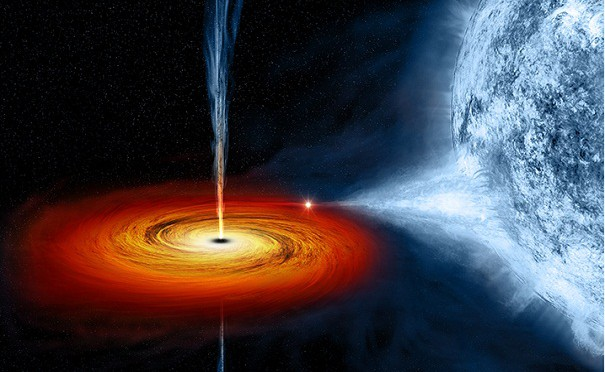
\includegraphics [width=\textwidth, angle=0.]{img/binaryaccretion.jpg}
    \end{center}
  \end{subfigure}
  \begin{subfigure}{.5\textwidth}
    \begin{center}
      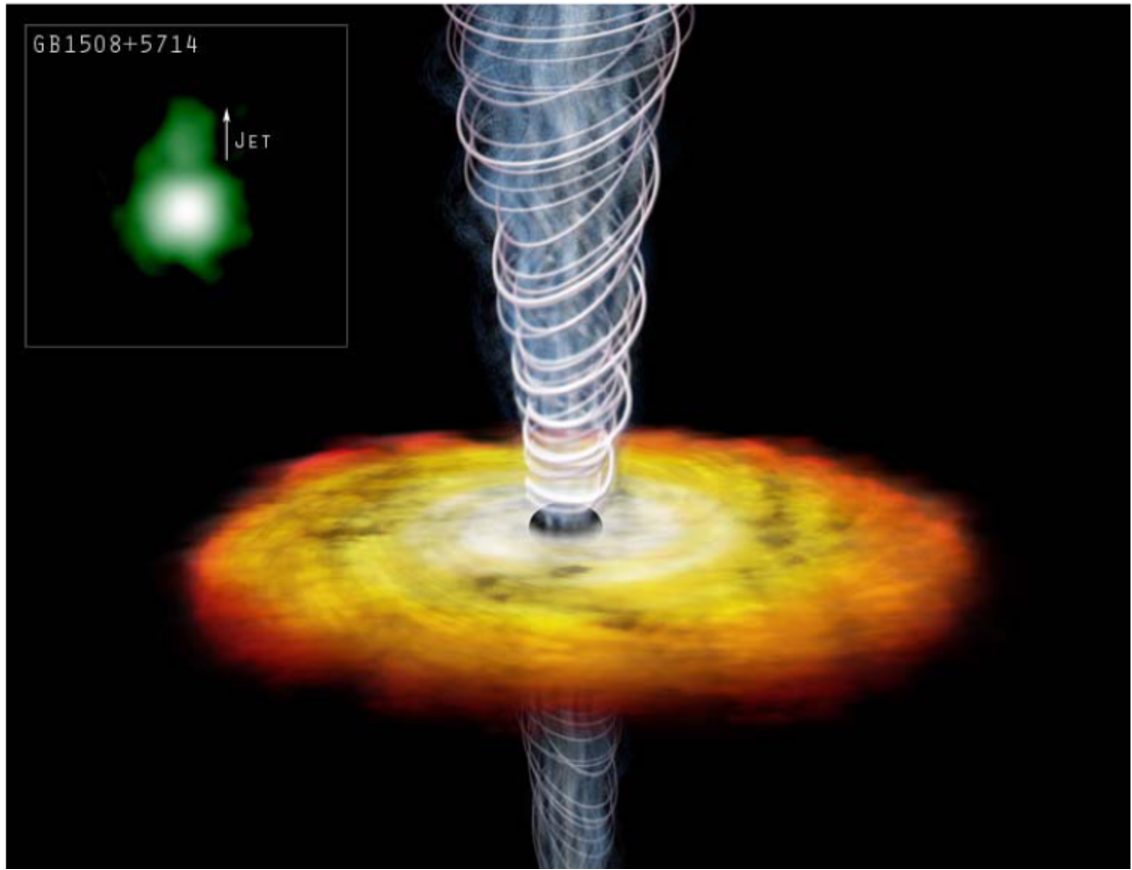
\includegraphics [width=\textwidth, angle=0.]{img/gb1508.pdf}
    \end{center}
  \end{subfigure}
  \caption{Artists' renderings of accretion disks. Left: accretion from a white dwarf onto a black hole. The accretion disk is in orange. Relativistic jets are shown launching out of the disk. Image from~\citet{Siemiginowska2003}. Right: around a supermassive black hole, supported by an image taken by the Chandra X-ray Observatory (inset). The disk itself is in orange, while magnetic field lines are shown in white around the collimated jets. Image from~\citet{Luminet2015}.}
  \label{fig:accdisks}
\end{figure}
\begin{table}[h]
  \centering
  \begin{tabular}{c|c|c|c|c|c|c}  
    & L (cm) & n (cm$^{-3}$) & T (eV) & B (G) & $\rho$ (cm) & $\lambda_{mfp}$ (cm) \\ \hline\hline
    ICM & 6.2e23 & 5.0e-3 & 8.0e3 & 1.0e-6 & 1.3e10 & 9.5e21 \\ 
    RIAFs & 3e17 & 1.0e2 & 2.0e3 & 1.0e-3 & 1e6 & 1e16  \\ 
    Solar wind & 1.5e13 & 1.0e1 & 1.0e1 & 1.0e-4 & 4.6e6 & 1.2e13  \\ \hline
    ISM & 3.1e20 & 1.0e0 & 1.0e0 & 5.0e-6 & 2.9e7 & 1.3e12  \\ 
    JET & 1.0e2 & 1.0e14 & 1.0e4 & 3.0e4 & 4.8e-1 & 1.4e6  \\ 
  \end{tabular}
  \caption{Comparison of parameters of different plasmas found in space and on earth. ICM: intracluster medium. ISM: interstellar medium. JET: Joint European Torus (a tokamak). Collisionless and weakly collisional plasmas are above the horizontal lines; collisional plasmas are below. Numbers calculated from parameters given in~\cite{Kunz2010,AST521Pset1}.}
  \label{table:paramCompare}
\end{table}


%--------------------------------------------------------------------%

\section{Motivation and Impacts}
This thesis will concentrate on weakly collisional plasmas in the context of RIAFs. This choice is motivated both by a recent paper that presents the first kinetic simulation of how accretion in a RIAF happens locally~\cite{Kunz2016} and by hints at the inability of a fluid model to capture the correct growth rates of kinetic phenomena~\cite{Sharma2004}. Although there has been some study on modified fluid closures to capture kinetic physics~\cite{Sharma2007,Sharma2003,SharmaThesis} especially by~\citet{Sharma2006}, henceforth referred to as~\citetalias{Sharma2006}, these studies use a different formalism and could only be compared to 2D simulations. Now that a 3D kinetic simulation has been performed by~\citet{Kunz2016}, hereafter referred to as~\citetalias{Kunz2016}, a direct comparison between a modified fluid closure and kinetic theory is possible. The paper uses methods that are easily replicated using the Athena code developed by~\citet{Stone2008}, in particular the same local shearing-box method~\cite{Stone2010}. A comparison is thus easily facilitated and meaningful. \\
\\
This paper is complementary to other current research in the field of accretion disk physics that often assumes a high degree of collisionality. For example, there is a push to include general relativity in accretion disk calculations in order to describe observations~\cite{Moscibrodzka2014,Ressler2015,Shiokawa2013,Sadowski2016,Niedzwiecki2014,Narayan1998,Gammie2003,Noble2006,Noble2009,Chan2015,Mocibrodzka2009}. This paper addresses the fundamental assumptions of these papers and assesses their validity, providing the groundwork for extending magnetohydrodynamics to relativistic systems and other effects.\\
\\
A fluid closure to kinetic physics has consequences beyond just black hole accretion. If proper parameters are found that sufficiently imitate the kinetic physics of RIAFs, then this model can be extended to global simulations and enables the exploration of the parameter space of other collisionless and weakly collisional plasmas. Such exploration is currently prohibitively expensive computationally as mentioned previously because PIC simulations are required. If a fluid model is achieved, then the simulations are much more manageable, allowing for more thorough scans of, for example, magnetic field strength. A fluid model closure to kinetic physics is also interesting in a conceptual sense since it would mean that the six phase-space degrees of freedom could be reduced to only three position-space degrees of freedom. \\
\\
The structure of this paper is as follows: the necessary background to understand the fundamental plasma physics question is explained in Chapter~\ref{sec:plasmaphysics}. The actual physical mechanism for accretion, a linear MHD instability called the magnetorotational instability (MRI), is outlined in Chapter~\ref{chap:compMRI} using both analytic theory and the main tool of the rest of this thesis---simulations. Building from the simplest MHD theory (ideal MHD) to more complex, resistive MHD, we transition into the original research of this thesis, found in Chapter~\ref{chap:kinbrag}. Chapter~\ref{chap:kinbrag} uses anisotropic viscosity along magnetic field lines in an attempt to capture kinetic physics with a modified fluid closure. 

